\documentclass[a4paper]{article}
\usepackage{vntex}
%\usepackage[english,vietnam]{babel}
%\usepackage[utf8]{vietnam}

%\usepackage[utf8]{inputenc}
%\usepackage[francais]{babel}
\usepackage{a4wide,amssymb,epsfig,latexsym,multicol,array,hhline,fancyhdr}

\usepackage{float}
\usepackage{amsmath}
\usepackage{lastpage}
\usepackage[lined,boxed,commentsnumbered]{algorithm2e}
\usepackage{enumerate}
\usepackage{color}
\usepackage{graphicx}							% Standard graphics package
\usepackage{array}
\usepackage{tabularx, caption}
\usepackage{multirow}
\usepackage{multicol}
\usepackage{rotating}
\usepackage{geometry}
\usepackage{xcolor}
\usepackage{longtable}
\usepackage{setspace}
\usepackage{epsfig}
\usepackage{tikz}
\usepackage{cite}
\usetikzlibrary{arrows,snakes,backgrounds}
\usepackage{hyperref}
\hypersetup{urlcolor=blue,linkcolor=black,citecolor=black,colorlinks=true} 
%\usepackage{pstcol} 								% PSTricks with the standard color package

\newtheorem{theorem}{{\bf Định lý}}
\newtheorem{property}{{\bf Tính chất}}
\newtheorem{proposition}{{\bf Mệnh đề}}
\newtheorem{corollary}[proposition]{{\bf Hệ quả}}
\newtheorem{lemma}[proposition]{{\bf Bổ đề}}


%\usepackage{fancyhdr}
\setlength{\headheight}{40pt}
\pagestyle{fancy}
\fancyhead{} % clear all header fields
\fancyhead[L]{
 \begin{tabular}{rl}
    \begin{picture}(25,15)(0,0)
    \put(0,-8){
\includegraphics[width=8mm, height=8mm]{hcmut.png}}
    %\put(0,-8){\epsfig{width=10mm,figure=hcmut.eps}}
   \end{picture}&
	%
\includegraphics[width=8mm, height=8mm]{hcmut.png} & %
	\begin{tabular}{l}
		\textbf{\bf \ttfamily Trường Đại Học Bách Khoa Tp.Hồ Chí Minh}\\
		\textbf{\bf \ttfamily Khoa Khoa Học và Kỹ Thuật Máy Tính}
	\end{tabular} 	
 \end{tabular}
}
\fancyhead[R]{
	\begin{tabular}{l}
		\tiny \bf \\
		\tiny \bf 
	\end{tabular}  }
\fancyfoot{} % clear all footer fields
\fancyfoot[L]{\scriptsize \ttfamily Bài tập lớn môn Lập trình hướng đối tượng
}
\fancyfoot[R]{\scriptsize \ttfamily Trang {\thepage}/\pageref{LastPage}}
\renewcommand{\headrulewidth}{0.3pt}
\renewcommand{\footrulewidth}{0.3pt}


%%%
\setcounter{secnumdepth}{4}
\setcounter{tocdepth}{3}
\makeatletter
\newcounter {subsubsubsection}[subsubsection]
\renewcommand\thesubsubsubsection{\thesubsubsection .\@alph\c@subsubsubsection}
\newcommand\subsubsubsection{\@startsection{subsubsubsection}{4}{\z@}%
                                     {-3.25ex\@plus -1ex \@minus -.2ex}%
                                     {1.5ex \@plus .2ex}%
                                     {\normalfont\normalsize\bfseries}}
\newcommand*\l@subsubsubsection{\@dottedtocline{3}{10.0em}{4.1em}}
\newcommand*{\subsubsubsectionmark}[1]{}
\makeatother


\begin{document}
\begin{titlepage}
\begin{center}
ĐẠI HỌC QUỐC GIA THÀNH PHỐ HỒ CHÍ MINH \\
TRƯỜNG ĐẠI HỌC BÁCH KHOA \\
KHOA KHOA HỌC - KỸ THUẬT MÁY TÍNH 
\end{center}

\vspace{1cm}

\begin{figure}[h!]
\begin{center}

\includegraphics[width=3cm]{hcmut.png}
\end{center}
\end{figure}

\vspace{1cm}


\begin{center}
\begin{tabular}{c}
\multicolumn{1}{l}{\color{blue}{{\textbf{{\Large LẬP TRÌNH HƯỚNG ĐỐI TƯỢNG}}}}}\\
~~\\
\hline
\\
\multicolumn{1}{l}{\color{blue}{\textbf{{\Large BÀI TẬP LỚN}}}}\\
\\
\color{blue}{\textbf{{\large ỨNG DỤNG TRÊN ĐIỆN THOẠI VỚI C\#}}}\\
\\
\hline
\end{tabular}
\end{center}

\vspace{3cm}


\begin{table}[h]
\hspace{5 cm}
\begin{tabular}{rll}
 GV: & Mai Đức Trung\\
\hline
  SV: & Nguyễn Huỳnh Minh & 1813085 \\
    & Võ Minh Long & 1812951 \\
     & Đoàn Ngọc Thịnh  & 1810542 \\
     
\end{tabular}
\end{table}

\vspace{2cm}
\begin{center}
{\footnotesize TP. HỒ CHÍ MINH, THÁNG 11/2019}
\end{center}
\end{titlepage}

\newpage
\tableofcontents
\newpage
\section{Giới thiệu}
\subsection{Giới thiệu về sản phẩm}
\hspace*{1 cm}Đây là sản phầm từ \textit{bài tập lớn} của môn \textbf{lập trình hướng đối tượng}, được thực hiện bởi nhóm \textit{Blue Stream}. Với hi vọng sẽ tạo ra một sản phẩm có ích và đáp ứng yêu cầu môn học, cả nhóm đã lên ý tưởng về việc tạo ra 1 ứng dụng chạy trên nền tảng điện thoại, cụ thể là \textit{Android}, vì tính phổ biến của nền tảng này. Cuối cùng, cả nhóm đã thống nhất sẽ làm 1 ứng dụng liên quan đến chính bản thân mỗi sinh viên, để hỗ trợ tốt hơn trong việc sắp xếp thời gian, cũng như học tập.\\
\hspace*{1 cm} Sản phầm này chỉ có sinh viên \textit{trường Đại học Bách Khoa TP.Hồ Chí Minh} mới có thể sử dụng được. Vì còn hạn chế về kĩ năng, kinh nghiệm, thời gian,... nên ứng dụng có những vấn đề chưa thật sự tốt, và như ý muốn.\\
\hspace*{1 cm}Ứng dụng được viết bằng ngôn ngữ lập trình \textit{C\#} với framework chính là \textit{Xamarin}, ngoài ra còn sử dụng \textit{SQLite}, \textit{Firebase} để lưu trữ dữ liệu,...
\subsection{Xamarin}
\subsubsection{Xamarin là gì?}
\subsubsection{Ưu điểm}
\subsubsection{Hạn chế}
\newpage
\section{Phân tích ứng dụng}
\begin{figure}[htp]
    \centering
    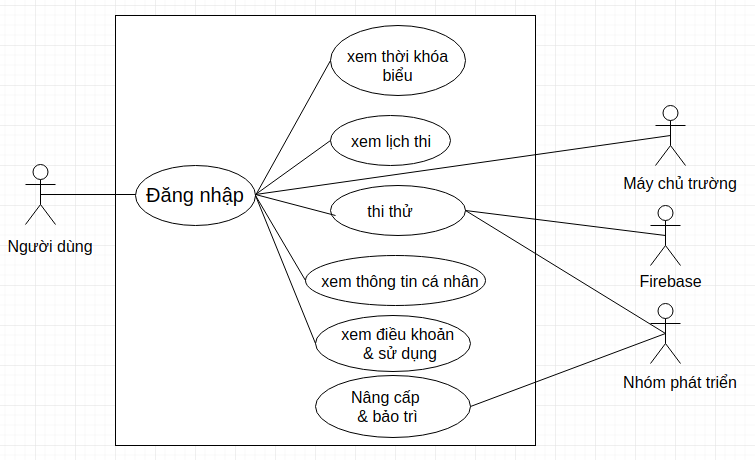
\includegraphics[scale = .35]{usecase.png}
    \caption{Bản vẽ Use Case của ứng dụng}
    \label{fig:usecase}
\end{figure}
Quan sát bản vẽ Use Case hình \ref{fig:usecase}, ta có thấy ứng dụng gồm có 6 khối chức năng chính mà người dùng có thể tương tác: đăng nhập, thời khóa biểu, lịch thi, thi thử, thông tin cá nhân, điều khoản & sử dụng. Chúng ta sẽ đi cụ thể vào từng khối.
\subsection{Yêu cầu}
\begin{itemize}
    \item Viết bằng ngôn ngữ lập trình \textit{C\#}
    \item Ứng dụng chỉ chạy trên nền tảng \textbf{Android phiên bản 5.0} trở lên.
    \item Phải có tài khoản \textbf{MyBK} của \textit{trường Đại học Bách Khoa TP.Hồ Chí Minh}
    \item Chạy tốt nhất trên các thiết bị có tỉ lệ màn hình $16:9$, cụ thể  là màn hình có độ phân giải $1280$x$720$
\end{itemize}
\subsection{Đăng nhập}
\hspace*{.5 cm}Đây là khối chức năng đầu tiên, cũng là bước quan trọng. Vì nếu không qua được khối này, thì người dùng không thể sử dụng các chức năng tiếp theo. Lưu đồ của khối này ở hình \ref{fig:login}. \\
\begin{figure}[H]
    \centering
    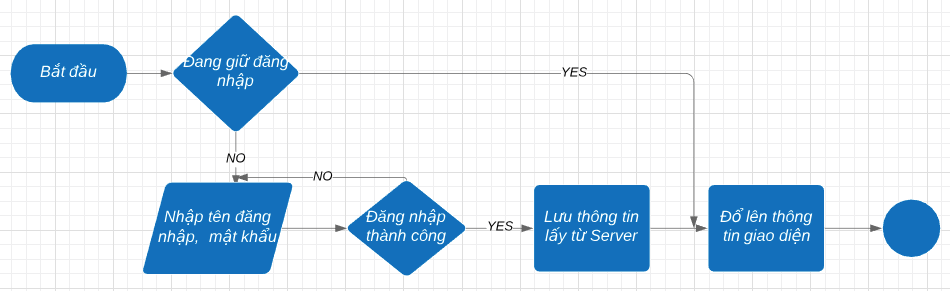
\includegraphics[scale=.4]{loginflow.png}
    \caption{Lưu đồ khối đăng nhập}
    \label{fig:login}
\end{figure}
\hspace*{.5 cm}Khi mới mở ứng dụng, đầu tiên sẽ kiểm tra nếu đã đăng nhập trước đó, và còn đang giữ trạng thái này, thì chỉ cần hiển thị lại thông tin đã được lưu lên giao diện. Ngược lại, thì người dùng cần cung cấp \textit{tên đăng nhập} và \textit{mật khẩu}. Nếu đăng nhập thành công, thì thông tin lấy được từ máy chủ gồm có: thời khóa biểu, lịch thi, thông tin cá nhân, dữ liệu câu hỏi sẽ được lưu lại. Rồi hiển thị các thông tin này lên giao diện, còn không thì phải nhập lại thông tin đăng nhập.
\subsection {Thời khóa biểu}
\hspace*{0.5 cm}Sau khi đăng nhập thành công, giao diện hiện ra đầu tiên là \textit{thời khóa biểu} của tuần học tương ứng. Dữ liệu được truy vấn từ \textit{database} lưu trên thiết bị. Lưu đồ cụ thể như hình \ref{fig:scheduler}.\\
\begin{figure}[h!]
    \centering
    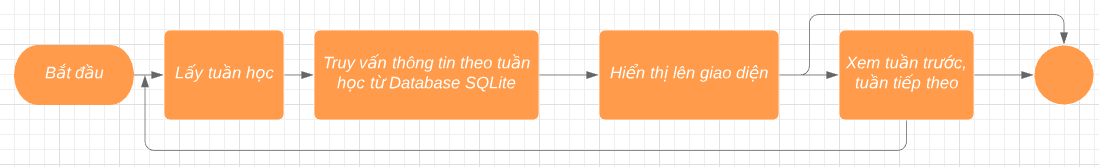
\includegraphics[scale=.4]{schedulerflow.png}
    \caption{Lưu đồ khối thời khóa biểu}
    \label{fig:scheduler}
\end{figure}\\
\hspace*{0.5 cm}Thời khóa biểu gồm có lịch học của nhiều tuần, nhưng ứng dụng chỉ hiển thị lịch học của tuần hiện tại theo từng ngày. Bên cạnh đó, người dùng cũng có thể xem lịch học của tuần trước hoặc tuần tiếp theo.
\subsection{Lịch thi}
\hspace*{.5 cm} Khối này gần giống với khối \textit{thời khóa biểu}. Lưu đồ cụ thể như hình dưới:
\begin{figure}[h!]
    \centering
    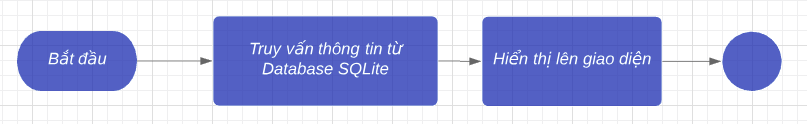
\includegraphics[scale=.4]{exam.png}
    \caption{Lưu đồ khối lịch thi}
\end{figure}\\
\hspace*{0.5 cm}Chức năng khối này đơn giản là lấy lại thông tin được lưu trên thiết bị, sau đó hiển thị lịch thi theo \textit{giữa kì} hay \textit{cuối kì}, và sắp xếp theo thứ tự diễn ra.
\subsection{Thi thử}
\hspace*{.5 cm} Đây là khối chức năng quan trọng, cũng là khá phức tạp hơn khi so với 3 khối trước. Lưu đồ cụ thể ở hình \ref{test}.
\begin{figure}[h!]
    \centering
    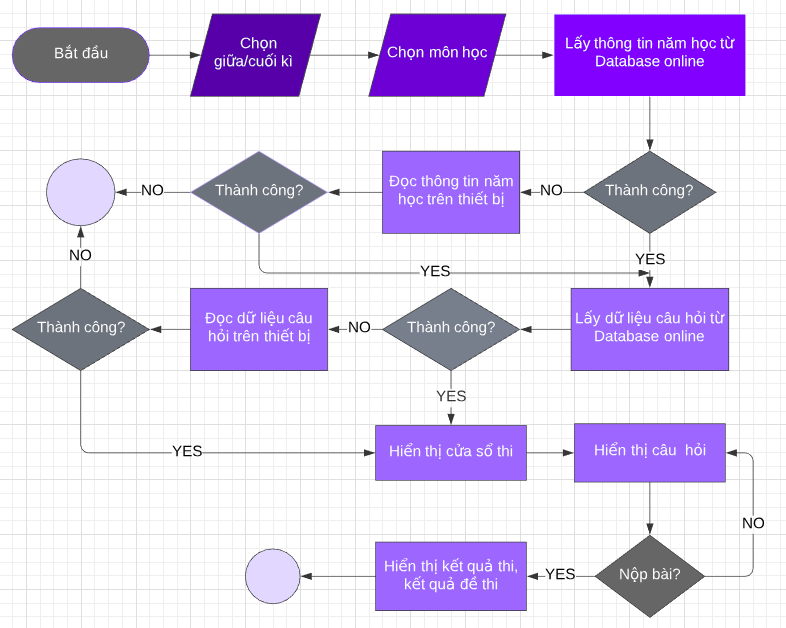
\includegraphics[scale=.4]{test.png}
    \caption{Lưu đồ khối thi thử}
    \label{test}
\end{figure}\\
\hspace*{0.5 cm}Ban đầu, người dùng cần chọn muốn thi thử giữa kì, hay cuối kì. Sau đó, sẽ hiện ra danh sách các môn học đang học trong kì đó, chọn tiếp 1 môn. Sau khi chọn xong, sẽ gửi yêu cầu lấy dữ liệu đến \textit{database online}, hoặc là \textit{dữ liệu lưu trên thiết bị}. Nếu quá trình này thành công, sẽ mở ra cửa sổ thi, hiển thị các câu hỏi, ngược lại thì sẽ thông báo \textit{'không có dữ liệu'}. Người dùng có thể nộp bài bất cứ lúc nào muốn để xem kết quả thi, và đáp án đề thi.
\subsection{Thông tin cá nhân}
\subsection{Khác}
\section{Thiết kế ứng dụng}
\subsection{Lược đồ lớp khối đăng nhập}
Lược đồ lớp khối đăng nhập cụ thể ở hình \ref{fig:uml_login}.
\begin{figure}[H]
    \centering
    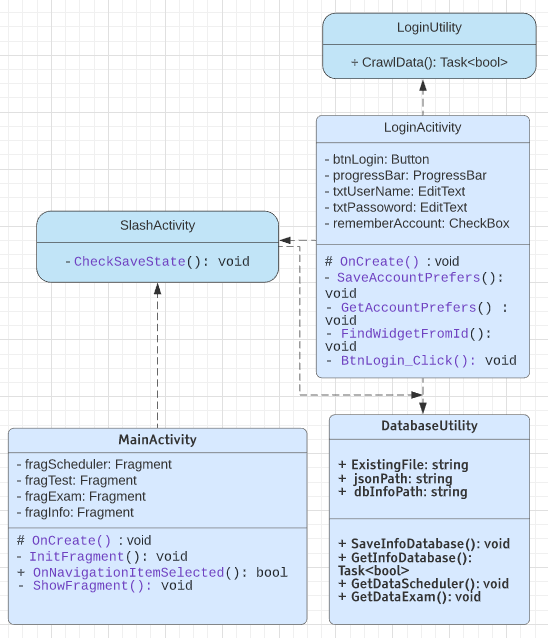
\includegraphics[scale = .5]{uml_login.png}
    \caption{Bản vẽ lớp khối đăng nhập}
    \label{fig:uml_login}
\end{figure}
\subsubsection{Lược đồ khối thời khóa biểu}
\end{document}